\documentclass[../Report.tex]{subfiles}
\graphicspath{ {../../Images/} }
\begin{document}
    \chapter{Ricerca Etnografica}
    \section{Segmentazione}
    Una piattaforma di gioco come gioco.it non riguarda le esigenze primarie di un bambino, potremmo quindi  identificarlo nel penultimo livello della piramide di Maslow: Stima del gruppo e auto-attualizazzione.
    Lo possiamo considerare come un momento di divertimento e di sfida in modo che possa permettere all’utente di qualunque etá di giocare alla piattaforma in modo sicuro, indipendentemente dall’età, specifiche del computer e interessi, poichè contiene una vastissima gamma di giochi. 
    Il sito, puó essere usato, oltre che per uno scopo ludico, per allenare le proprie capacitá di problem solving, la creativitá ed per apprendere nuove nozioni su tantissimi temi.

    \subsection{Segmentazione Demografica}
    
    Non esiste una specifica distinzione a priori tra soggetti per un gruppo demografico maschile o femminile poiché il sito si rivolge ad entrambi i sessi. Cercheremo tuttavia però di distinguere gli utilizzatori attraverso la loro età:
    \begin{itemize}
        \item Bambini (4-12): primi approcci ad un computer, potrebbero essere interessati anche a giochi di tipo educativo
        \item Adolescenti (12-18): il sito può essere utilizzato sopratutto nel tempo libero da ragazzi che utilizzano un computer, spesso durante le pause dallo studio. 
        \item Adulti (18 +): i genitori sono target del sito come "accompagnatori" dei dei figli di età più piccola che neccessitano di supporto al computer. Inoltre sono responsabili dei tempi di utilizzo e delle scelte di giochi dei loro bambini. Non è escluso un utilizzo anche di questo segmento di utenti come utilizzatori poichè sono presenti sul sito molti giochi che non hanno limiti di età e sono degli ottimi passatempi anche per soggetti adulti. 
    \end{itemize}

    Illustriamo attraverso il seguente grafico alcune considerazioni intuitive tra il rapporto di età di un utente, il tempo libero che un individuo possiede e il tempo di utilizzo del nostro servizio. 
    È una stima indicativa per evidenziare il target di utenti piu adatto su cui focalizzarci.
    Assumiamo che la fascia 5-10/10-18 sia quella con maggior tempo libero a disposizione e con predisposizione tale da utilizzare il nostro servizio, la fascia di mezzo (30-60) è quella con minor tempo libero, di conseguenza, con il minor tempo di utilizzo ed infine la fascia over 65 il tempo libero aumenta ma questo non influisce sul tempo di utilizzo di una piattaforma di giochi online, che resta è veramente ridotto e spesso limitato ove possibile al controllo di utilizzo di figli e nipoti. 

    \begin{figure}[H]
        \centering
        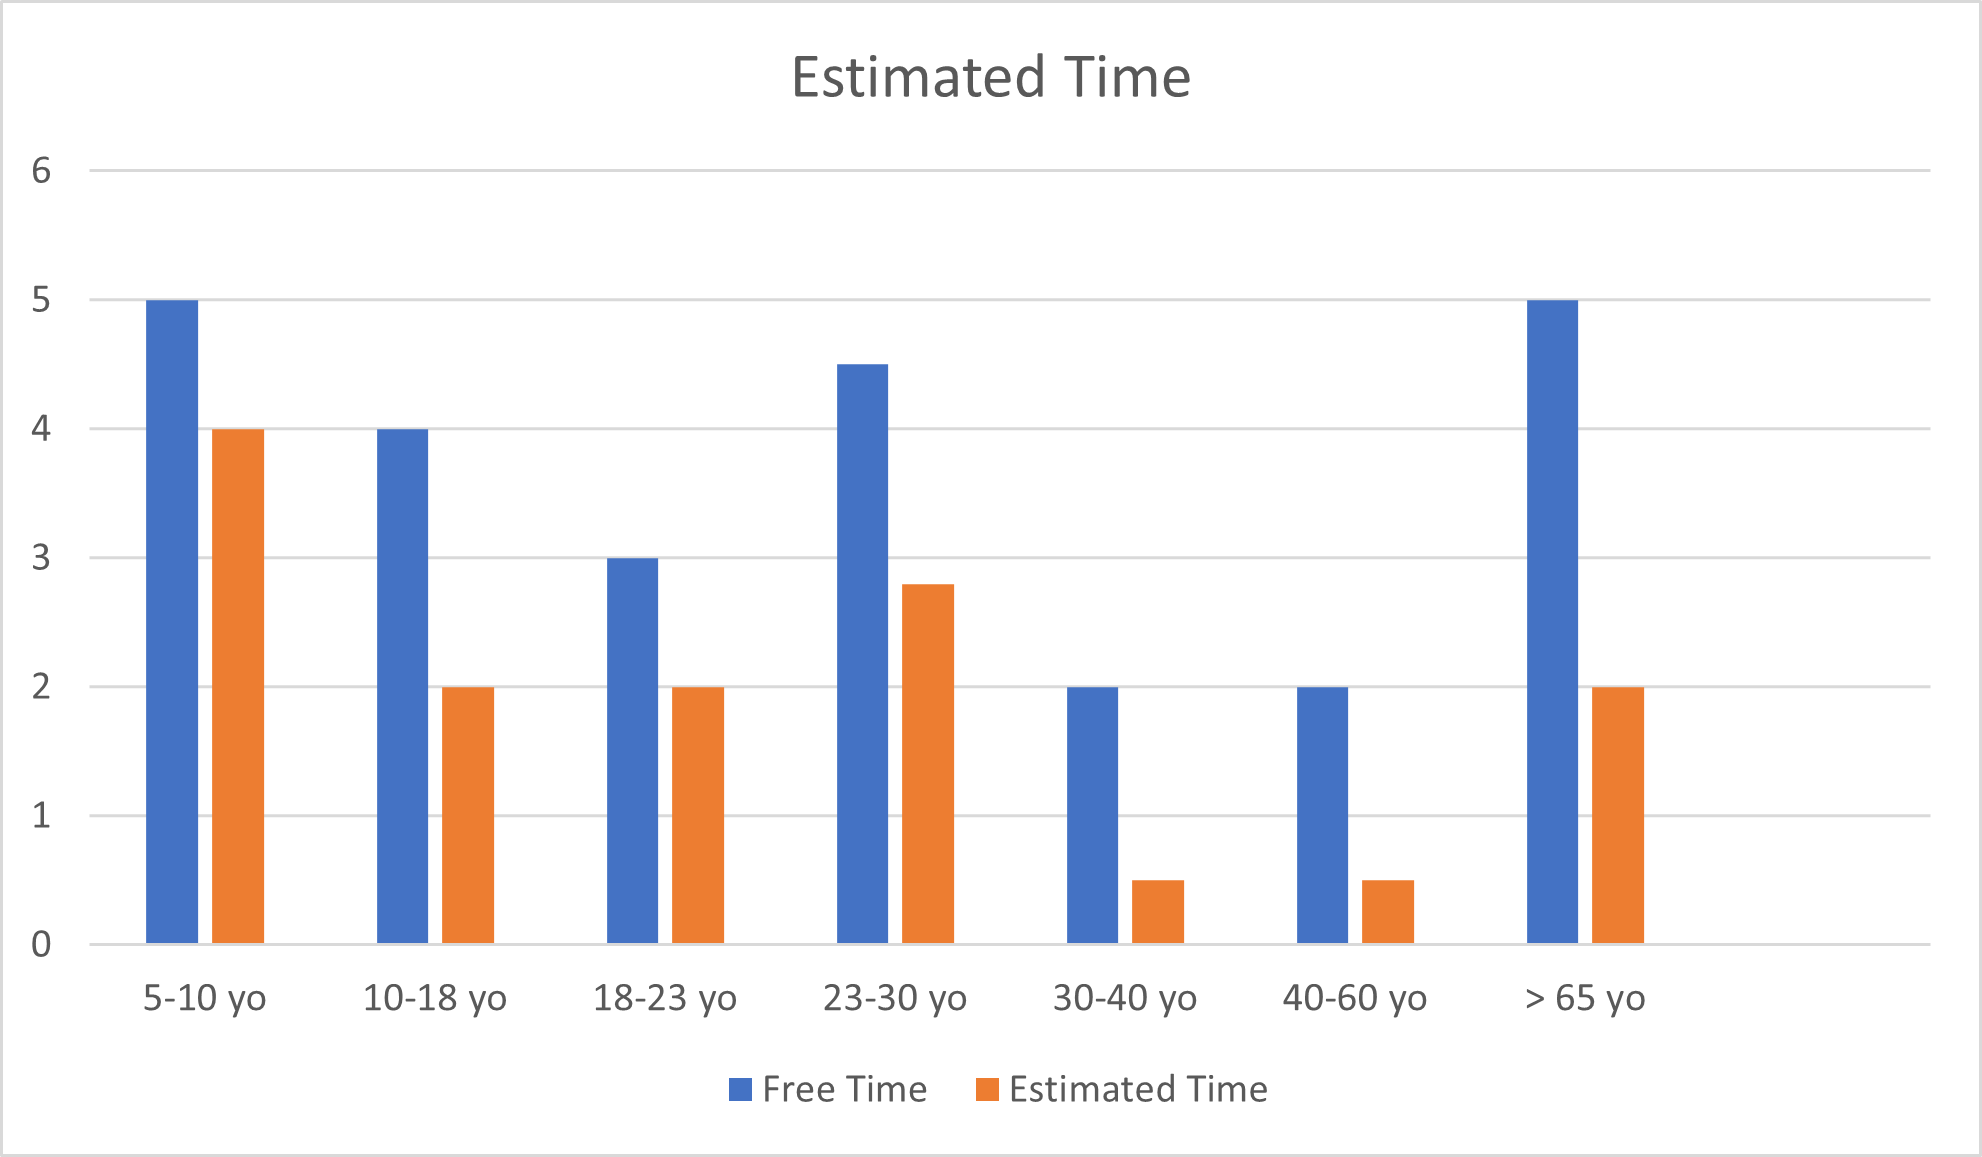
\includegraphics{EstimatedTime.png}
    \end{figure}

    Nel prossimo grafico invece mostreremo una stima delle competenze in ambito informatico in base alle differenti fasce d’eta, distinguendo le ‘Competenze’ tra base (accendere/spegnere un computer, navigare nel dekstop, controllare la mail), medie (scaricare applicazioni, utilizzare un word processor e fogli di calcolo) e alte (ottima familiaritá con l’utilizzo dei computer).

    \begin{figure}[H]
        \centering
        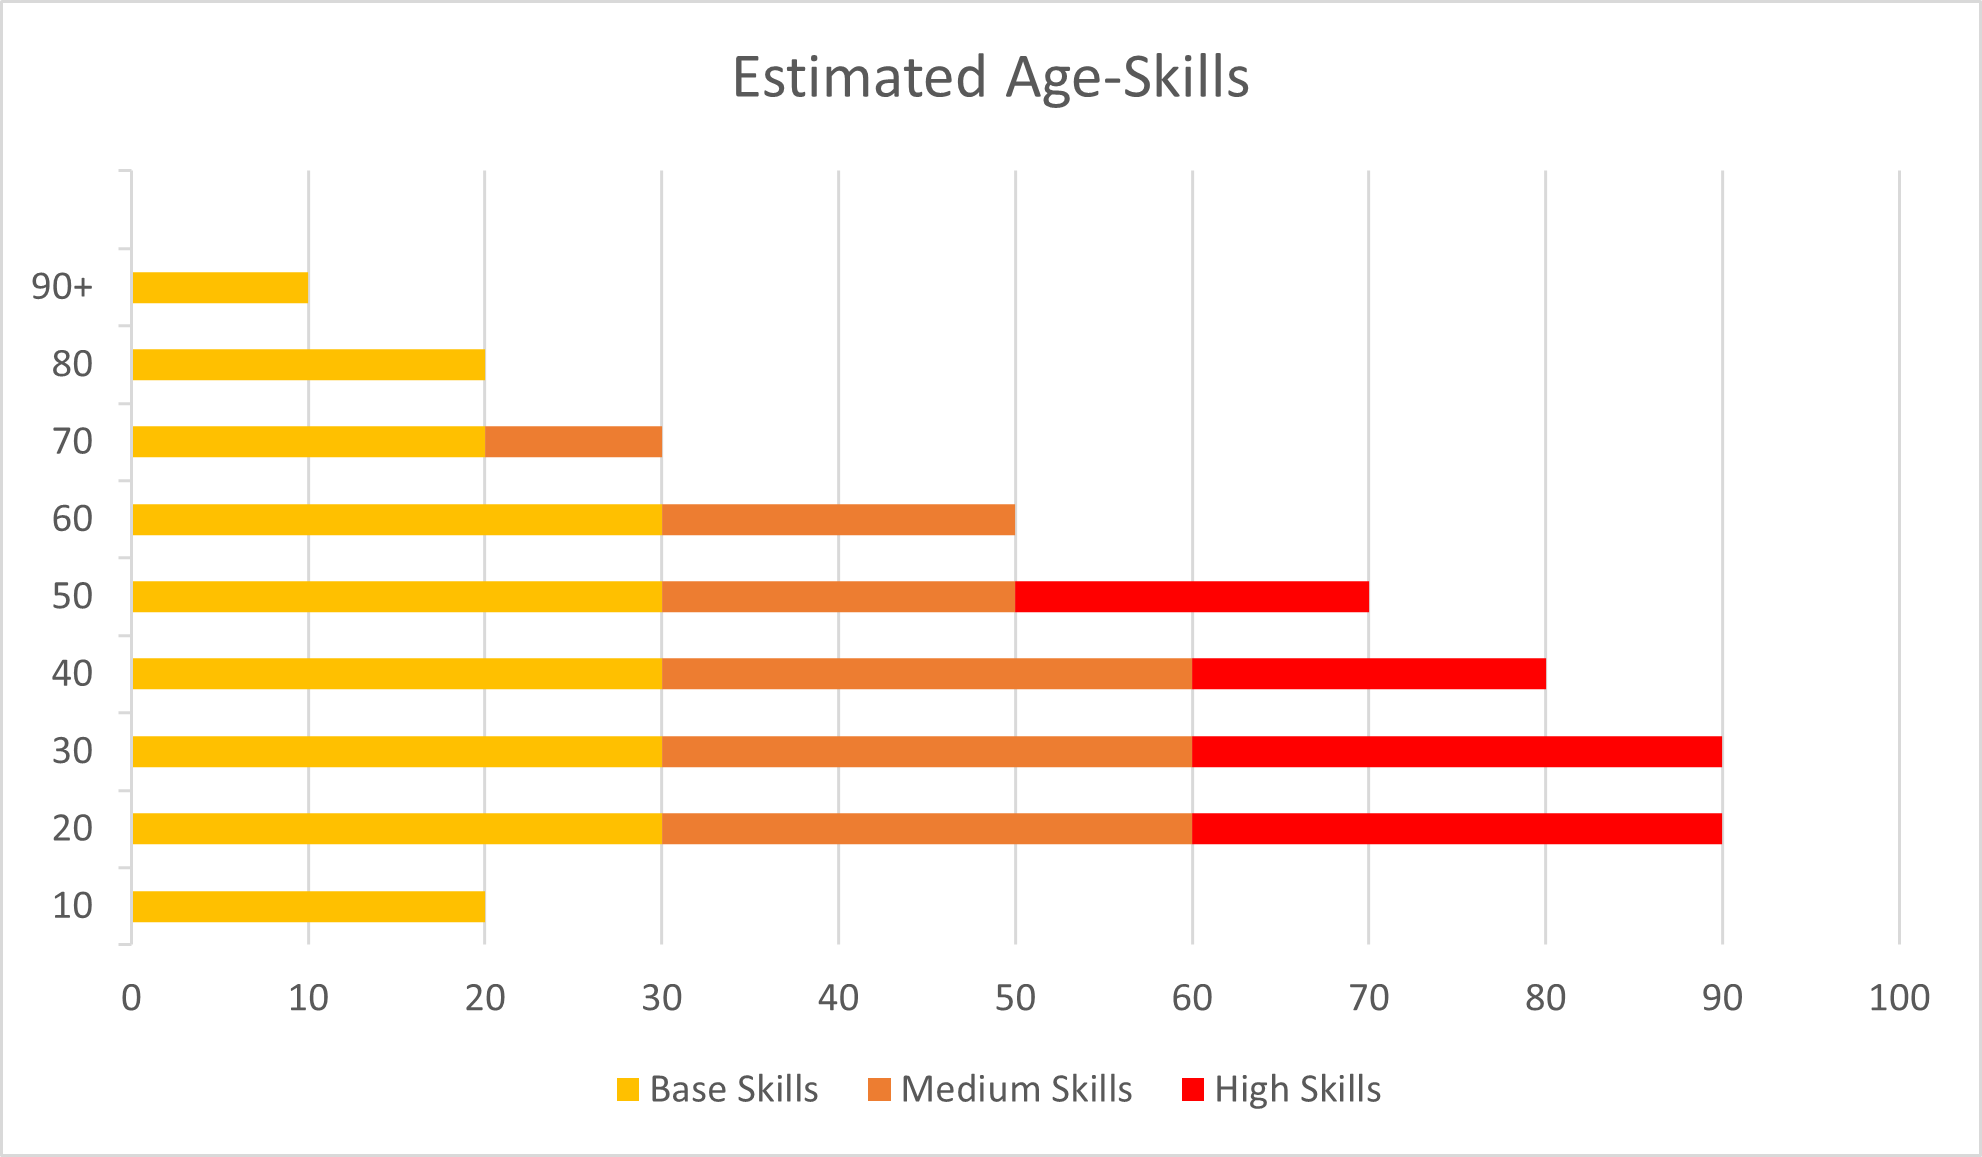
\includegraphics{EstimatedAgeSkills.png}
    \end{figure}

    Intuitivamente possiamo capire che le persone tra 20-40 anni possiedono in media piú competenze e abilitá nell’utilizzo dei computer mentre troviamo piú difficolta nelle due fasce estreme di età (troppo piccoli o troppo anziani).
    
    \subsection{Segmentazione Psicografica}

    Non ci sono dei veri e propri tratti psicografici distintivi che possono caratterizzare l'utilizzo o meno del sito. Risulta pero, chiaro ammettere come bambini e ragazzi che preferiscano rimanere a casa e siano più introversi passano molto più tempo al computer e di conseguenza su Gioco.it rispetto a bambini e ragazzi che preferiscono attivitità motoria o attività all'aperto. 
    Non avendo una segmentazione demografica netta l’interfaccia dovrà conciliare i gruppi di età degli utenti di diverse età proponendo descrizioni, giudizi di altri utenti in modo da rendere il gruppo di utenti sempre più ampio (fattore molto utile per quanto riguarda la possibilità del multiplayer) e la possibilità di sfruttare l'effetto \emph{rich-get-richer}.

    \subsection{Segmenti Target}
    Identifichiamo così possibili segmenti target:
    \begin{itemize}
        \item Bambini (3-12 anni): soggetti che non sono in grado da soli di utilizzare al meglio un computer e che utilizzerebbero il sito principalmente per giocare, divertirsi e imparare accompagnati da un genitore.
        \item Adolescenti (12-18 anni): soggetti che utilizzano autonomamente il sito per giocare e divertirsi durante il loro tempo libero. 
        \item Adulti (18+ anni): soggetti che utilizzano il sito principalmente come supervisori per soggetti più piccoli (figli o fratelli minori), preoccupandosi delle loro scelte e aiutandoli nei task da effettuare. Rimane comunque la possibilità che possano utilizzare il sito come fruitori di contenuto per divertirsi e passare del tempo.       
    \end{itemize}

    \section{Ricerca Utenti}
    
    La nostra ricerca sugli utenti consiste in interviste con campioni di utenti scelti dai nostri dati demografici.\\
    In questa sezione il nostro obiettivo è determinare:
    \begin{itemize}
        \item Se i segmenti provvisori della sezione precedente rispondono bene all’idea alla base del nostro e costituiscono un buon pubblico di destinazione
        \item Evidenziare le principali aspettative degli utenti target per quanto riguarda l’utilizzo della piattaforma
    \end{itemize}

    
    \subsection{Interviste}
    Descriviamo la nostra ipotetica piattaforma ai nostri intervistati e poniamo loro una serie di domande riguardanti l’argomento:
   
    \begin{enumerate}
    \item Hai buona familiarità con l’utilizzo dei computer e dei sistemi informatici?
    \item Hai mai giocato su internet in una piattaforma di giochi online?
    \item Pensi che vorrai utilizzare il servizio?\\
         In caso affermativo\\
        \begin{enumerate}
            \item Quando pensi che potresti utilizzare il servizio?\\ 
             In caso negativo: 
            \item Come mai?
            \item Chi pensi possa essere più adeguato ad utilizzare questo servizio?
        \end{enumerate}
    \item	Quali pensi possano essere i vantaggi più significativi di questo servizio?
    \item	Quali pensi possano essere gli svantaggi di questo servizio?
    \item	Pensi che ci possa essere qualche preoccupazione nell’utilizzo della piattaforma da utenti minorenni?
    \end{enumerate}
    \subsection{Metodo di indagine}
    Tutte le interviste sono state svolte di persona direttamente da noi, in qualità di membri del team di design. Il colloquio è stato assolutamente informale per mettere gli intervistati più a loro agio possibile.
    
    \subsection{Risultati}
    \textbf{Intervistato A}

    \textbf{Nome}:Sofia\\
    \textbf{Eta'}:36\\
    \textbf{Professione}:Impiegata
    
    \begin{enumerate}
        \item Buona familiarità con l’utilizzo degli strumenti informatici dovuto ad un forte utilizzo in ambito lavorativo. Lavora tutti i giorni al pc ed utilizza principalmente strumenti e programmi di produttività. 
        \item Si, ha giocato spesso su internet (sopratutto ai giochi presenti su Facebook) e vede spesso i suoi figli (6 e 12 anni) giocarci. 
        \item Probabilmente si, per riempire tempo libero oppure per far giocare i figli con scopi educativi.
        \item Il principale vantaggio è il fatto che i bambini possano apprendere divertendosi. 
        \item Il principale svantaggio è legato al grado di dipendenza che i bambini possano manifestare in relazione ad una piattaforma come questa. 
        \item No, serve però un’attenzione da parte dei genitori per fare in modo che i filtri non vengano ignorati e aggirati dai bambini.
    \end{enumerate}

    Note: Di solito per cercare questo tipo di giochi guarda i primi risultati delle ricerche su Google\\

    \hrule
    \textbf{Intervistato B}

    \textbf{Nome}:Gianni\\
    \textbf{Eta'}:63\\
    \textbf{Professione}:Libero Professionista
    
    \begin{enumerate}
        \item Scarsa conoscenza dei sistemi informatici, usa il telefono per rispondere a chiamate di lavoro.
        \item Non ha mai giocato sui giochi di piattaforma online però ha visto i suoi figli (15 e 23 anni) giocarci. Molto raramente ha aiutato i suoi figli nell'utilizzo, lascia questo compito a sua moglie. 
        \item Non crede ci giocherebbe date le competenze informatiche limitate, ha un computer a casa ma viene usato principalmente da sua moglie e i suoi figli. \\Pensa che sarebbe piú adeguato un pubblico piú giovane che abbia maggior conoscenza dei sistemi informatici.
        \item Il fatto che i giochi siano gratuiti e liberamente accessibili. 
        \item Il piú grande svantaggio potrebbe essere che molte recensioni possano essere false per aumentare la visibilitá di un determinato gioco.
        \item Potrebbero esserci delle preoccupazioni legate al tempo di utilizzo da parte dei bambini di queste piattaforme.  
        
    \end{enumerate}
    \hrule
    \textbf{Intervistato C}\\
    
    \textbf{Nome}:Fabrizio\\
    \textbf{Eta'}:38\\
    \textbf{Professione}:Operaio

    \begin{enumerate}
        \item Limitata conoscenza de computer, utilizza solo lo smartphone per chiamare, mandare messaggi e navigare sui social network
        \item Si, sui giochi online dei social network quale Facebook per sfidare i suoi amici. 
        \item Gli piacerebbe prendere dimestichezza con i computer, in caso contrario potrebbe provare a far giocare il figlio (8 anni) se avesse la sicurezza di giocare in un ambiente "sicuro".
        \item Pensa che il vantaggio principale sia avere per ogni gioco una descrizione e una valutazione fornita da altri utenti, che possano quindi darne un primo feedback sulla qualità. 
        \item Crede che il principale svantaggio sia legato al controllo, e al fatto che i propri figli possano giocare a giochi non adatti alla loro età.
        \item Non crede, dato che pensa che le recensioni di altri utenti possano difficilmente essere surreali.
    \end{enumerate}

    \hrule
    \textbf{Intervistato D}\\

    \textbf{Nome}:Sara\\
    \textbf{Eta'}:23\\
    \textbf{Professione}:Studentessa universitaria

    \begin{enumerate}
        \item Buone competenze digitali dovuto ad un assiduo utilizzo in universita e a casa.
        \item Si, diverse volte sopratutto quando è in pausa dallo studio. Ha anche dichiarato di aver in passato utilizzato direttamente il sito Gioco.it quando aveva tra i 13 ed i 16 anni. Inoltre, essendo Sara una babysitter afferma di aver fatto usare il sito Gioco.it alle bambine che accudisce, per trovare qualche momento in più per rivedere gli appunti delle lezioni. 
        \item Sì, però solo nei momenti liberi (pausa studio o noia) se il suo computer fosse gia acceso. Afferma che  non accenderebbe mai il computer per utilizzare la piattaforma.
        \item Il fatto che sia accessibile da piu dispositivi e non servono requisiti e competenze avanzate puo essere un punto favorevole.
        \item Crede che il sito sia troppo ricco di giochi, alcuni copie di altri. 
        \item Crede che possano esserci problemi poiché l'attuale filtro per i giochi accessibili dai maggiorenni è facilmente aggirabile.
        
    \end{enumerate}

    \hrule
    \textbf{Intervistato E}\\

    \textbf{Nome}:Lucia\\
    \textbf{Eta'}:44\\
    \textbf{Professione}:Insegnante delle elementari

    \begin{enumerate}
        \item Buona familiaritá con l’uso dei computer dovuto ad un uso quotidiano durante l’orario scolastico e al di fuori di esso per uso personale.
        \item Non ha mai giocato su questo tipo di piattaforme ma potrebbe essere utile da far giocare agli studenti magari per giochi a scopo educativo e durante l’ora di laboratorio di informatica.
        \item Userebbe il servizio nel suo tempo libero per fare esperienza, testarlo per farne poi un uso didattico a scuola.
        \item Il vantaggio principale è la presenza di giochi educativi.
        \item Il fatto che non si possa stilare un ranking tra un determinato gruppo di utenti, che le permetterebbe di creare "competizioni" nella classe.
        \item Non crede che l’utilizzo di questo servizio da parte di studenti minorenni controllati da un adulto possano destare preoccupazioni. Diverso è il suo punto di vista se non ci fosse un controllo adulto. 
    \end{enumerate}
    
    \hrule
    \textbf{Intervistato F}\\
    \textbf{Nome}:Leonardo \\
    \textbf{Eta'}:62\\
    \textbf{Professione}:Ex Militare in Pensione

    \begin{enumerate}
        \item Ha una conoscenza sufficiente dei sistemi informatici. Sa utilizzare la mail, fa ricerche sul web ed è iscritto ai principali social media per restare in contatto e vedere gli aggiornamenti dei suoi figli, trasferiti al Nord Italia. 
        \item Utilizza raramente Gioco.it assieme alle sue nipotine quando si fermano a casa sua in vacanza. 
        \item Dichiara che personalmente non utilizzerebbe mai una piattaforma del genere e preferirebbe fare, anche con le sue nipotine, attività più manuali. Dichiara però che cede volentieri all'utilizzo del sito quando le sue nipotine glielo chiedono con dolcezza. 
        \item Crede che il principale vantaggio sia la grande quantità di giochi. 
        \item E' spaventato dal fatto che le sue nipotine possano passare troppo tempo davanti ad uno schermo, piuttosto che fare attività più manuali come la pasta fatta in casa. 
        \item E' molto preoccupato dal fatto che utilizzando il sito abbia visto che siano presenti anche giochi non adatti a bambini, come Slot Machine e giochi violenti.    
    \end{enumerate}
    
    \newpage
    \subsection{Conclusioni}

    Notiamo che le interviste hanno confermato la validitá dei nostri dati demografici e psicografici, poiché la maggior parte  degli intervistati hanno espresso interesse nell’uso del servizio o un interessamento allo stesso.
    Inoltre, da queste interviste possiamo risaltare una lista di casi d’uso provvisori che ci mettono in evidenzia il ‘perché’ un utente debba utilizzare il nostro servizio, e troviamo:
    \begin{itemize}
        \item Motivi di svago e distrazione
        \item Motivi Educativi
    \end{itemize}
    Abbiamo focalizzato la nostra attenzione su utenti target del servizio, riferendoci per lo più a genitori o educatori. 
    Da un’osservazione delle interviste degli utenti abbiamo notato inoltre che:
    \begin{itemize}
        \item Un gioco deve essere ben descritto, avere delle chiare immagini esemplificative e avere delle recensioni veritiere.
        \item La schermata deve essere intuitiva, l’utente usa il servizio e gioca per un periodo limitato di tempo; deve essere invogliato a scegliere il miglior gioco nel minor tempo possibile.
        \item Di solito i genitori che accompagnano i figli nel gioco non sono abili nell’uso dei computer, bisogna quindi semplificare l'utilizzo del sito. 
        \item Molti soggetti si dicono preoccupati della presenza di giochi non adatti all'età dei loro bambini. 
        \item I genitori non vogliono che il sito possa creare una sorta di dipendenza nei bambini e preferiscono che il tempo di utilizzo resti limitato. 
    \end{itemize}
    

    \subsubsection*{Altre Idee}
    Dalle interviste, tuttavia, sono venute fuori particolari funzionalitá che potrebbero essere aggiunte in futuro:
    \begin{itemize}
        \item Avere una sezione contenenti le classifiche dei giochi piu utilizzati e in base alla valutazione degli utenti
        \item Possibilitá di connettere un gruppo di amici, ed eventualmente stilare le varie classifiche 
        \item Limitare il tempo di gioco di un utente minorenne sotto la supervisione di un genitore
        
    \end{itemize}



\end{document}